\section{Vorgehen}
In diesem Kapitel wird das Vorgehen der Projektgruppe detailliert dargestellt. Dabei soll als Struktur der Prozess der Softwareerstellung verwendet werden. Es gilt also zunächst die Phase der Modellierung zu beschreiben und anschließend die eigentliche Softwareentwicklung zu erläutern. Ebenso wird in diesem Kapitel dokumentiert, wie der Routing-Algorithmus entwickelt wurde und welche Komplexitäten im Rahmen dessen aufgetreten sind.

\subsection{Modellierung}
Zur Betrachtung der Wirtschaftlichkeit eines energieeffizienten Netzes muss ein Vergleich zwischen einem Standardnetz (Business-As-Usual-Netz) und einem energieeffizienten Netz durchgeführt werden. Bei der Spezifikation des Netzes liegt ein Hauptaugenmerk auf der Eingrenzung des Netzes. Im Rahmen dieser Arbeit soll dabei nur das Core-Netz betrachtet werden. Der eingerahmte Bereich aus Abbildung \ref{fig:VorgModNetz} beinhaltet die \textquote{Broadband Network Gateway} (BNG), \textquote{Label-Switch-Router} (LSR) und \textquote{Label-Edge-Router} (LER).


\begin{figure}[htb]
	\centering
	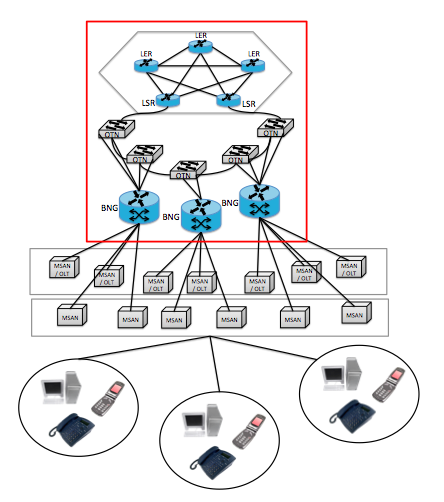
\includegraphics[width=0.8\textwidth]{VorgModNetz}
	\caption{Eingrenzung des Netzwerks} 
	\label{fig:VorgModNetz}
\end{figure}


Damit ein Vergleich möglich ist, müssen beide Netze identisch modelliert werden. Das statische Netz soll in der Simulation nicht  verändert werden. Das zweite Netz soll die im Kapitel \ref{SdF} beschriebenen Technologien anwenden und die Effizienz des Netzes damit zu steigern. Um sowohl das Standard als auch das effiziente Netz möglichst realistisch zu modellieren, sollen die Geräte pro Layer gewählt werden. Die Geräte werden dann in der Datenbank konfiguriert.  Die Modellierung des Netzes erfolgt durch die Erstellung von Verbindungen zwischen den Geräten in Abhängigkeit von der Netzlastverteilung. Zuvor muss eine Anzahl von Knoten im Netz definiert und ein Netzlastprofil erstellt werden.

\begin{figure}[htb]
	\centering
	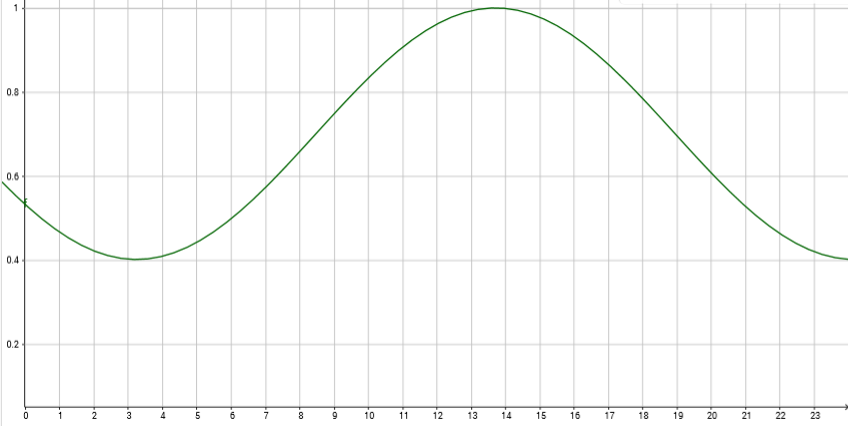
\includegraphics[width=0.8\textwidth]{VorgModLast}
	\caption{Idealtypische Netzlast-Kurve (nach \cite[3]{Chiaraviglio2009})} 
	\label{fig:VorgModLast}
\end{figure}

Die in Abbildung \ref{fig:VorgModLast} gezeigte Sinuskurve stellt die Netzwerklast dar. Die Abbildung ist eine Anlehnung an ein realitätsgetreues Netzwerklastprofil. In der Fallstudie \cite[1]{Chiaraviglio2009} werden die Daten eines großen italienischen Internet Service Providers verwendet, um ein realistisches Netzwerklastprofil zu erstellen und damit die Energieeinsparung durch energieeffiziente Technologien zu berechnen.

Die Kurve aus Abbildung \ref{fig:VorgModLast} hat ihren Tiefpunkt um kurz nach 3 Uhr nachts. Um diese Zeit wird die geringste Datenlast durch das Netz geroutet. Morgens steigt die Kurve an, bis gegen 13:30 Uhr der Höhepunkt erreicht wird. Danach sinkt die Sinuskurve wieder dem Tiefpunkt entgegen. Dieser Verlauf wiederholt sich jeden Tag. Der Höhepunkt gegen halb 2 Uhr nachmittags ist damit zu begründen, dass zu dieser Zeit die meisten Menschen auf der Arbeit oder im Privaten Anwendungen nutzen, die über das Internet betrieben werden oder das Internet nutzen. Nachts schlafen die meisten, weshalb im diesem Zeitraum weniger Traffic über das Netz geroutet wird. 

\subsection{Entwicklung des Routing-Algorithmus}\label{subsec:VorgAlg}
In teilvermaschten Telekommunikationsnetzen können mehr als nur ein Weg durch das Netzwerk von der Datenquelle zum Ziel führen. Wie beispielsweise in \ref{fig:VorgAlgNetzrouting} zu erkennen ist, kann ein einzelner Netzknoten nicht ohne zusätzliches Wissen über die Anordnung und Kapazitäten der anderen Netzelemente zum jetzigen Zeitpunkt die \"beste\" Entscheidung zur Weiterleitung treffen. Das gleiche Problem muss auch in der Entwicklung eines Routing-Algorithmus beachtet werden. \ref{fig:VorgAlgNetzrouting} stellt ein Modell eines Carrier-Netzwerkes bestehend aus Knoten (Router oder Switches) und Kanten (eine oder mehrere Verbindungen) dar. Daten sollen von dem Quell-Knoten zum Senke-Knoten geleitet werden. Quell- und Senke-Knoten liegen außerhalb des Carrier-Netzwerkes des betrachteten Telekommunikationsnetzwerkes.

Zur Simulation des Netzwerkes, der Lastverteilung und zur Berechnung des elektrischen Stromverbrauches des Netzwerkes ist ein iterativer Ansatz notwendig. Jede Iteration stellt einen Zeitabschnitt dar, für den mehrere Datenströme, definiert durch eine Netzlast, den Traffic-Ursprung (Quelle) und das Traffic-Ziel (Senke), durch das Netz geleitet werden. Die iterative Berechnung erlaubt die getrennte Bestimmung des Stromverbrauches für jeden Zeitraum. Dies ermöglicht die Beachtung der Uhrzeit-abhängigen Belastung der Carrier-Netze und darauf basierend das An- oder Ausschalten von Netzkomponenten zur Steigerung der Energieeffizienz des Carrier-Netzes.  

\begin{figure}[htb]
	\centering
	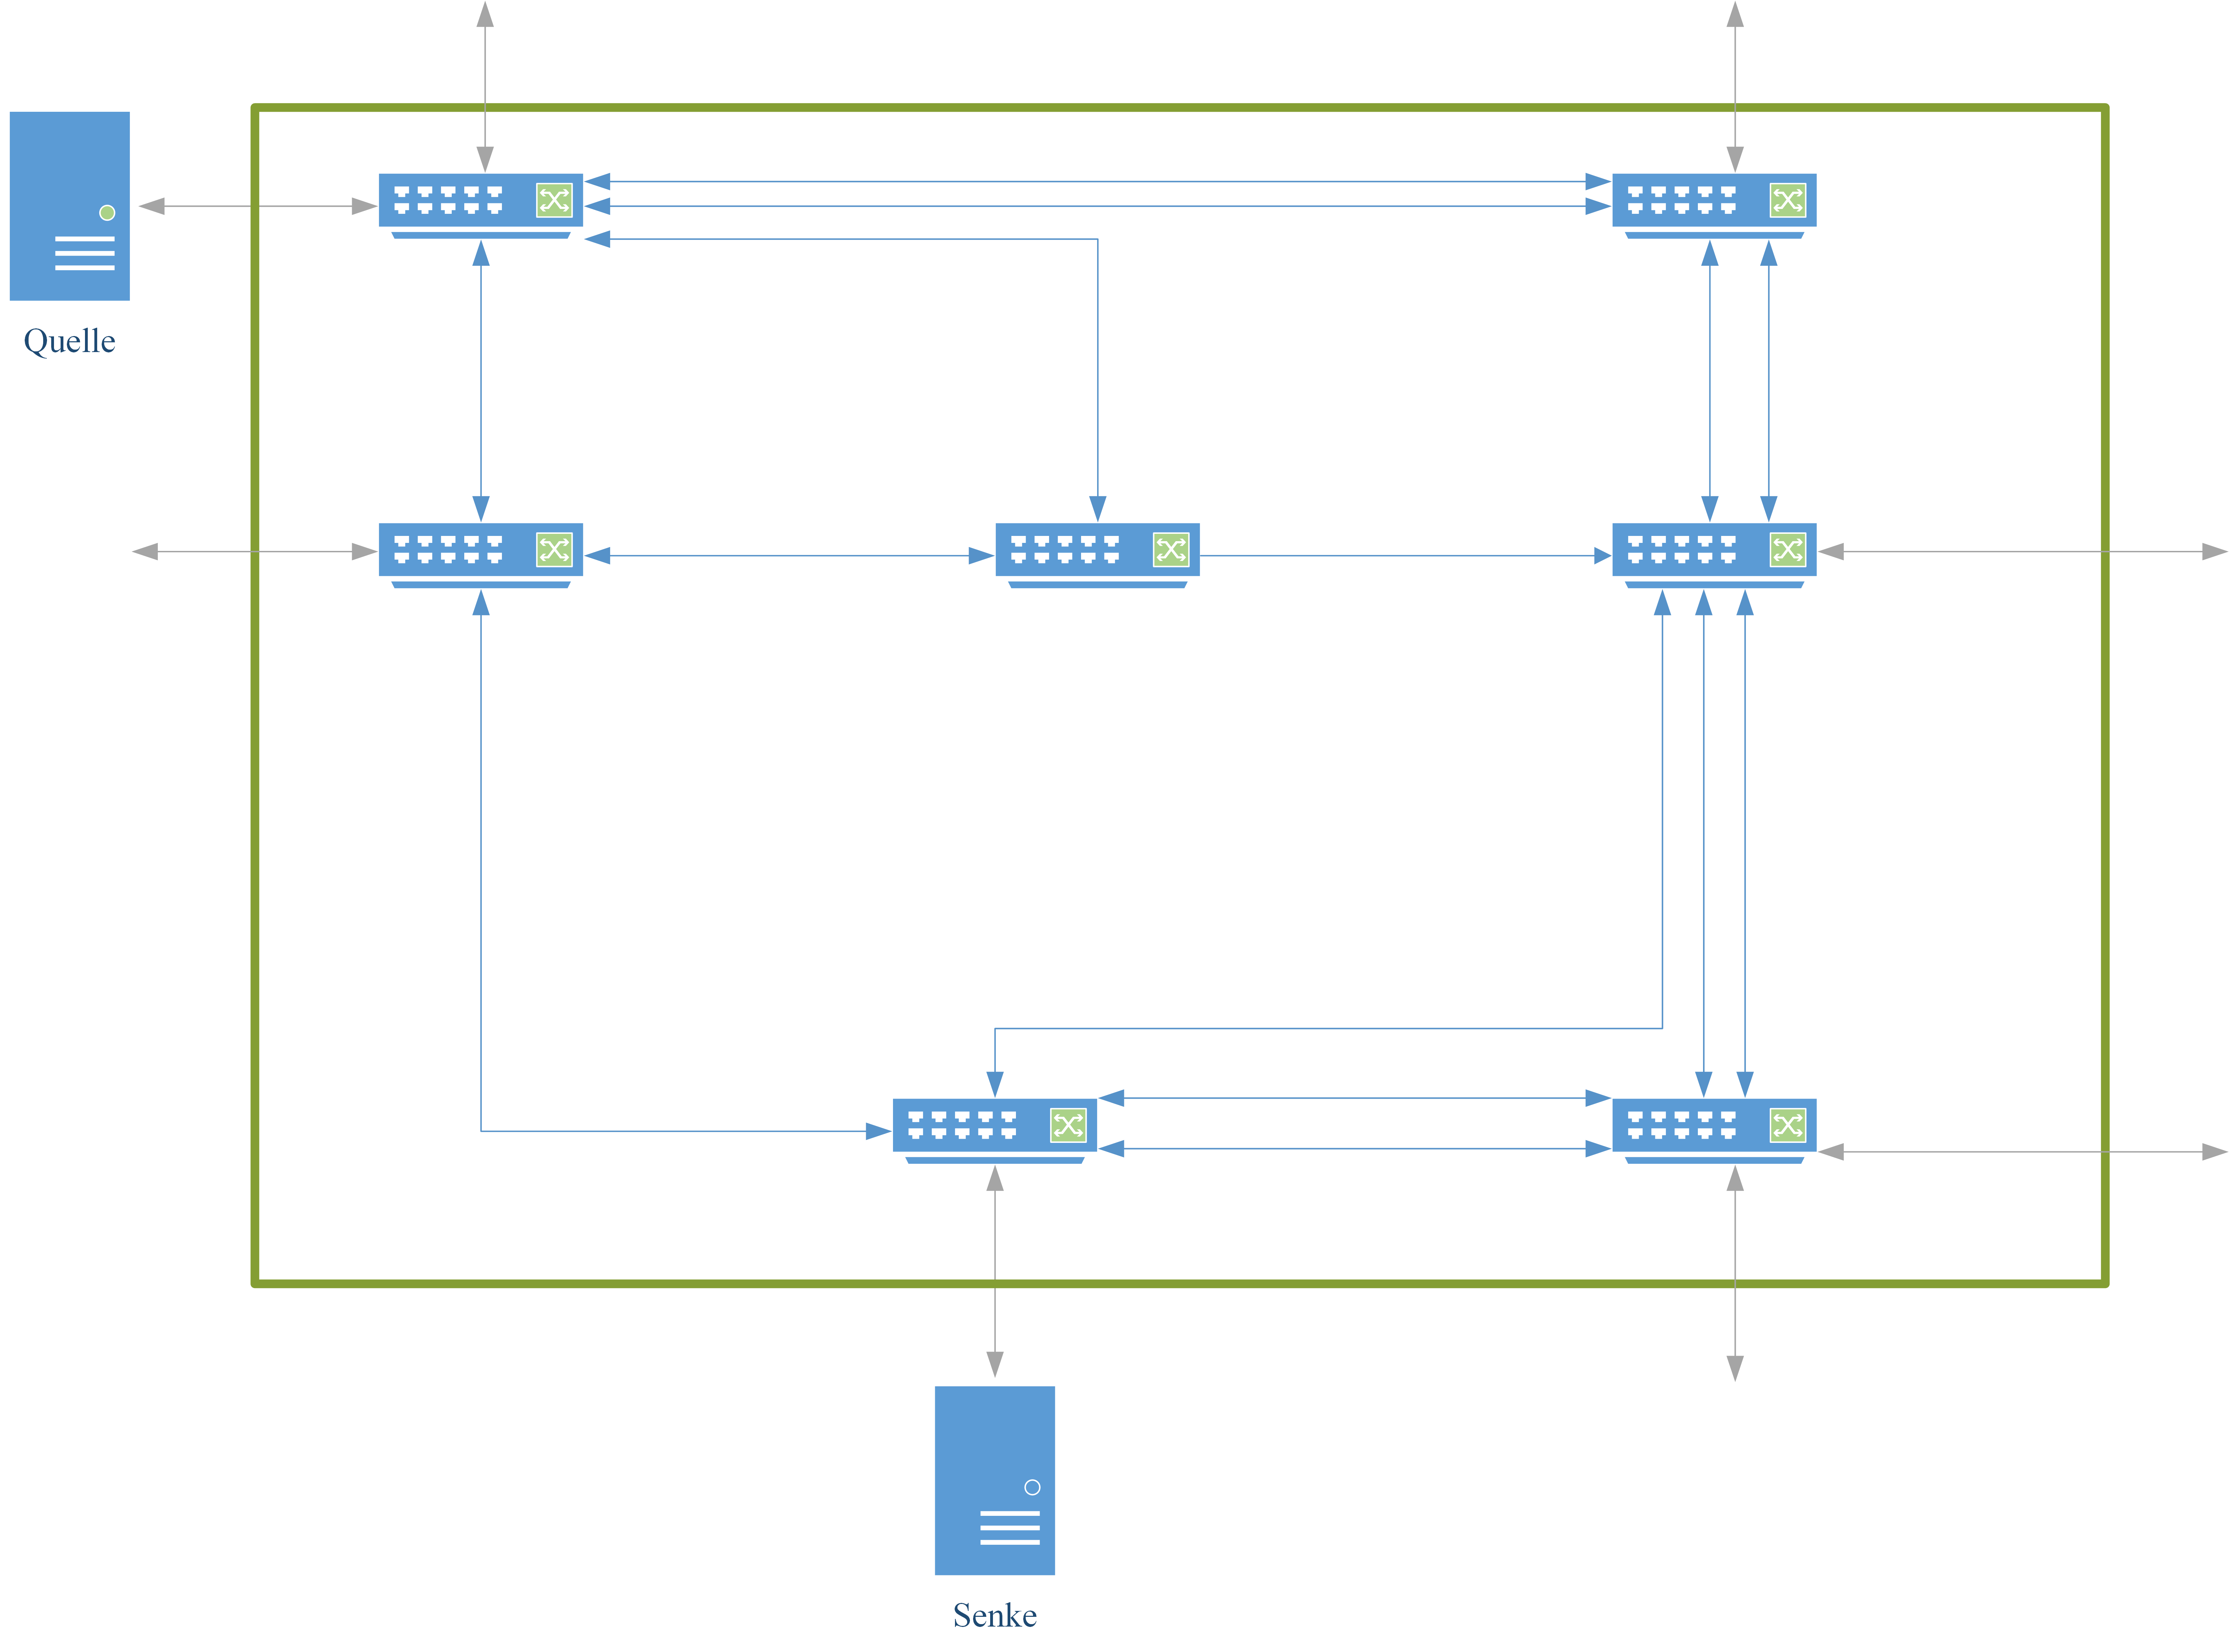
\includegraphics[width=\textwidth]{VorgAlgNetzrouting}
	\caption{Modellnetz mit mehreren Routingmöglichkeiten}
	\label{fig:VorgAlgNetzrouting}
\end{figure}

Es stehen zur Berechnung des Stromverbrauchs eines Zeitabschnitts generell mehrere Ansätze zur Verfügung. Der logisch einfachste Ansatz wäre es, von einer bestimmten zuvor als Datenbankeintrag festgelegten Nutzungsauslastung pro Verbindung auszugehen (feste Werte bezüglich Auslastung je Gerät). Dies würde ein einfaches Bestimmen der einzelnen Geräte\-aus\-las\-tungen und anschließendem Addieren der Werte zu einem Gesamtstromverbrauch pro Zeiteinheit ermöglichen. Diese Ergebnisse könnten dann als Tabelle und Histogramm dargestellt werden.

Dieser Lösungsweg setzt allerdings eine sehr detaillierte und statische Modellierung eines Beispielnetzes und allen dazugehörigen Auslastungs- und Verbrauchswerten je Zeitabschnitt voraus. Aufgrund dieses Konfigurationsaufwands wird ein Anwender folglich einen großen Zeitraum für eine Iteration auswählen, was zu einer sehr groben und realitätsfernen Simulation führen würde. Energiespartechniken, wie das dynamische Abschalten von einzelnen Verbindungen und Umrouten der Netzlast auf andere noch nicht optimal ausgelastete Verbindungen, muss der Anwender in diesem Verfahren selbstständig für jede Iteration umsetzen.

Als zweite Möglichkeit zur Berechnung der optimalen Stromverbrauchswerte bietet sich das automatisierte, in einem Algorithmus implementierte Berechnen der einzelnen Netz\-last-Routing-Mög\-lich\-kei\-ten an. Aus allen möglichen Wegen für ein Netzlast-Element kann anschließend, nach einem zuvor definierten Regelsatz, das am besten geeigneten Routing ausgewählt werden.

Ein solcher Algorithmus bietet den Vorteil, dass der Anwender neben dem Netzaufbau nur die Netzlast mit Iterationszeitraum, Quelle, Senke und Menge spezifizieren muss. Die Software errechnet aus diesen Daten selbstständig eine für das gesamte Problem akzeptable Lösung bestehend aus den einzelnen Routing-Entscheidungen.

Dieser Greedy-Algorithmus liefert nicht für jeden Anwendungsfall die beste Lösung, da für jede Entscheidung nur ein einzelnes Netzlast-Element betrachtet wird.
Würden für jede Iteration stattdessen auch die Wechselwirkungen zwischen den Routingmöglichkeiten betrachtet, wäre die Berechnung wesentlich aufwändiger und zeitintensiver.
Ein weiterer Nachteil eines solchen Algorithmus ist, dass dieser nicht die im Netz des Anwenders verwendeten Regeln zum Routing nachahmt, sondern das Netz als teilvermascht mit Gleichberechtigung der einzelnen Strecken bei Anwendung des fest implementierten Regelsatzes betrachtet.
Die Implementierung eines Algorithmus, der alle Spezialitäten des Netzes des Anwenders beachtet, würde den Rahmen dieser Arbeit wesentlich überschreiten. Eine evolutionäre Erweiterung des zuvor beschriebenen Algorithmus um durch den Anwender zu spezifizierende Regelsätze ist als Weiterentwicklung dieser Arbeit allerdings möglich.

Der im Rahmen der vorliegenden Arbeit entwickelte und in Kapitel \ref{subsec:ErgAlg} beschriebene Algorithmus bedient sich des dynamischen Routings der Netzströme und ist somit in die zweite Kategorie einzuordnen.

\subsection{Softwareentwicklung}\label{subsec:VorgSoftwareEng}
Die zuvor beschriebene Modellierung zur Kalkulation und Simulation von energieeffizienten Netzen soll im nächsten Schritt softwaretechnisch umgesetzt werden. Als Vorgehensmodell hat sich das Projektteam am Wasserfallmodell mit den folgenden Entwicklungsstufen orientiert:
\begin{itemize}
\item Anforderungsanalyse
\item Spezifikation
\item Systemdesign
\item Implementierung
\item Test
\end{itemize}

\subsubsection{Anforderungsanalyse}
Die Analyse der Anforderungen an die Simulationssoftware erfordert eine zielgerichtete Recherche über bereits vorhandene Technologien und Methoden. Ebenfalls müssen die Funktionalitäten, die das Simulationstool bereitstellen soll, abgegrenzt werden. Die Anforderungen werden zunächst als Ideen und Möglichkeiten gesammelt und dann in Form von Anforderungsspezifikationen definiert. 

Das System soll ein statisches Netz mit einer festgelegten Anzahl an Verbindungen abbilden. Alle Daten zu Geräten, Netzen, Verbindungen und Netzprofilen sollen in einer MySQL-Datenbank gespeichert werden. Die Verwendeten Geräte sowie neue Netzprofile sollen über die Datenbank eingepflegt werden können. Für das Netzprofil sollen Traffic-Daten (Netzprofil, Last, Quelle, Senke, Uhrzeit) verwendet werden. Aus den Daten entsteht eine gleichbleibende Auslastungskurve, anhand derer die Verbindungen für die jeweilige Uhrzeit definiert werden können. Um das Netz möglichst realistisch zu simulieren bekommen die einzelnen Verbindungen eine Länge zugeordnet. Anhand dieser Länge (mehr als 80 km) wird definiert, ob ein Verstärker hinzugefügt werden muss, um die Verbindung zu verbessern. Das definierte, statische Netz soll die Verwendung verschiedener Technologien und Methoden zur Senkung des Energieverbrauchs möglich machen. Zur Abschaltung von Switches und Ports soll ein Algorithmus entwickelt werden, der auf dem \textquote{Exhaustive Greedy Algorithm} aus \cite{fisher} aufbaut.

\subsubsection{Spezifikation}
Im Zuge der Anforderungsanalyse und der Spezifikation der Software wurden die folgenden funktionalen, nicht funktionalen und datenbezogenen Anforderungen erstellt:



Funktionale Anforderungen:
\begin{itemize}
	\item A1: Über die Datenbank kann ein Netz, bestehend aus Knoten (Geräte) und Kanten (Verbindungen) modelliert werden
	\item A2: Das Anlegen neuer Geräte und Geräte\-konfi\-gura\-tionen ist über die Datenbank möglich
	\item A3: Das Verändern von Geräte\-parametern ist über die Datenbank möglich
	\item A3a: Das Austauschen von Geräte\-typen ist über die Datenbank möglich
	\item A3b: Das Austauschen von Geräte\-typen pro Schicht ist über eine GUI möglich                       
	\item A4: Das System berechnet anhand des modellierten Netzes, der eingestellten	Geräte\-konfi\-gura\-tionen, der gewählten Energiespartechnologien und des vorliegenden Lastprofils den Stromverbrauch.
	\item A5: Das System berechnet die Stromkosten anhand des Stromverbrauches und eines vorgegebenen Umrechnungsfaktors 
	\item A6: Zur Vereinfachung von Berechnungen müssen Annahmen getroffen werden, die in der Datenbank hinterlegt werden
	\item A7: Es werden generische Geräte basierend auf \cite{vanhsheet} verwendet
	\item A8: Zur Abschaltung von Switches/Ports dient der \textquote{Exhaustive Greedy Algorithm}
	\item A9: Der simulierte Stromverbrauch im Laufe eines Tages soll pro Stunde graphisch ausgegeben werden
	\item A10: Die Lastkurve wird graphisch dargestellt
\end{itemize}


Nicht funktionale Anforderungen:
\begin{itemize}
	\item NFA1: Das System soll nur als Client-Applikation vorliegen
	\item NFA2: Das System verwendet eine MySQL-Datenbank als Persistenzschicht
\end{itemize}


Datenbezogene Anforderungen:
\begin{itemize}
	\item DA1: Verbindungen wird eine Länge zugewiesen
	\item DA2: Für Gerätetypen können relevante Leistungs- und Verbrauchsparameter hinterlegt werden
	\item DA3: Ein Netz entsteht durch das Verbinden von Geräteinstanzen
	\item DA4: Annahmen werden durch einen eindeutigen Namen und einen Wert abgebildet
	\item DA5:  Die Netzlast wird in Form von Datenpaketen mit den Attributen Volumen, Quelle, Senke, Uhrzeit, Profil-ID definiert
\end{itemize}

\subsubsection{Systemdesign}\label{subsubsec:VorgSoftDesign}
In der Systemdesign-Phase werden einige Entscheidungen bezüglich der Softwareentwicklung getroffen. Als Programmiersprache für das Projekt wurde objektorientiertes Java ausgewählt. Die bereits vorhandene Entwicklungserfahrung im Team mit der Programmiersprache und der sehr guten Verfügbarkeit von kostenfreien Entwicklungstools und fertigen Bibliotheken waren für die Entscheidung ausschlaggebend.
Die Architektur besteht aus einer 2-Tier Kombination aus einer relationalen MySQL/MariaDB Datenbank und einer Fat-Client Anwendung. Die Datenbank wird dabei zur Speicherung der zur Erstellung eines Netzes notwendigen Daten, sowie Hardware-, Topologie- und Netzwerkkonfiguration verwendet. Die Anwendung hingegen wird zur Parameterkonfiguration, Berechnung der Zielwerte und Ausgabe der Resultate verwendet.


Die Vorteile der Architektur sind die gute Portabilität der resultierenden Lösung und die Ermöglichung einer einfachen und schnellen Entwicklung. Es müssen keine weiteren Anwendungsserverkomponenten je Entwicklungsumgebung installiert und konfiguriert werden. Die SQL-Datenbank verwendet eine übliche Datenbank-Standardsoftware und kann per SQL-Script vollautomatisch konfiguriert werden.
Das Datenbank-Konzept ist entscheidend für die Softwareentwicklung. Es werden alle relevanten Daten für Berechnungen, Konfigurationen und Darstellungen gespeichert. Auf der Basis der Datenbankstruktur kann die Entwicklung der Softwarelösung weitergeführt werden.


\begin{figure}[htbp]
	\centering
	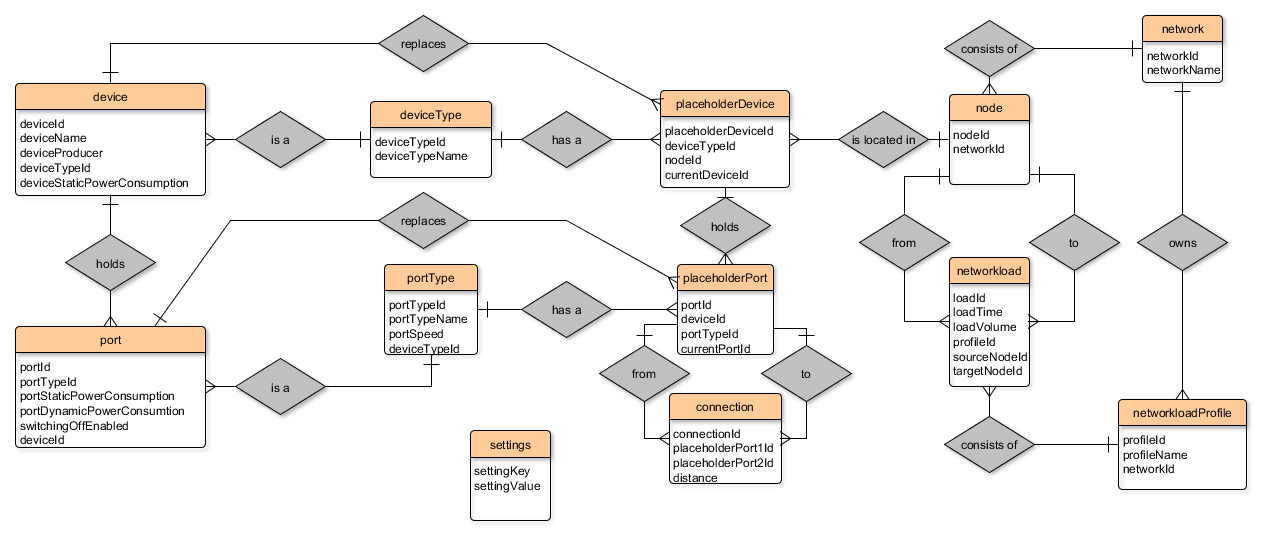
\includegraphics[width=0.9\textwidth]{VorgSoftwareER}
	\caption{ER-Diagramm} %TODO Bezeichnung anpassen
	\label{fig:VorgSoftwareER}
\end{figure}

In Abbildung \ref{fig:VorgSoftwareER} ist das Entity-Relationship-Modell für die Software zur Simulation der Netzwerke zu sehen. In der Tabelle \textquote{device} können Netzwerkkomponenten hinterlegt werden, die durch Attribute in \textquote{deviceType} und \textquote{port} um weitere Informationen ergänzt werden. Diese Geräte werden für die in \textquote{placeholderDevice} festgelegten Platzhalter eingesetzt, wobei sich einer oder mehrere Platzhalter in einem Netzknoten, einer \textquote{node}, befinden kann. Mehrere Platzhalter in einem Netzknoten sind beispielsweise nötig, um die Geräte der verschiedenen Layer dort hinterlegen zu können. Über \textquote{connections} sind die Ports der Platzhaltergeräte miteinander verbunden.

Ebenfalls jeweils einem Netzwerk zugeordnet sind die Netzlastprofile (\textquote{networkloadProfile}), da die darin enthaltenen Netzwerklast-\textquote{Pakete} mit je einem konkreten Start- und Ziel-Netzknoten verbunden sind. Die Tabelle \textquote{settings} beinhaltet alle Annahmen und Einstellungen, die für die Berechnung und Darstellung notwendig sind. 

\subsubsection{Implementierung}
In der Programmierungsphase wurde ein Grundgerüst für die weitere Entwicklung der Software geschaffen. Die Datenbank wurde auf der Basis des zuvor erstellten Konzeptes eingebunden. Im Rahmen der Weiterentwicklung kann der Routing-Algorithmus und die definierten Anforderungen implementiert werden. Der Algorithmus koordiniert das Routing des Traffics durch das definierte Netz. Mit der Hilfe von weiteren Annahmen und Algorithmen kann die Software zu einem System entwickelt werden, das verschiedene Technologien und Methoden zur Energiereduzierung einsetzt. Das Programm könnte die verschiedenen Methoden möglichst realitätsgetreu anwenden und die dadurch gesparte Energie graphisch darstellen. Über die GUI könnte eine Konfiguration möglich sein.  Darüber könnten verschiedene Technologien aktiviert und Geräte ausgetauscht werden. 

Um den Energieverbrauch im Carrier-Netzwerk berechnen zu können, werden für jede verwendete Netzkomponente Parameter wie Portanzahl, Geschwindigkeit und Stromverbrauch benötigt. Innerhalb der Simulation wird für die Berechnung des Gesamtverbrauchs auf die definierten Werte zurückgegriffen, die in einer Datenbank gespeichert sind. Deren Schema wurde so definiert, dass Werte beispielsweise aus \cite{vanhedde} genutzt werden können. Die Quelle beinhaltet zum einen das analytische Modell der Berechnung und zum anderen ein Datenblatt \cite{vanhsheet} des Energieverbrauchs der unterschiedlichen Hersteller. Das Datenblatt gliedert die Geräte in die Layer IP/MPLS, Ethernet, OTN und WDM (OSI-Layer: 3-2-1-1). Zu beachten ist beim Verwenden der Werte, dass es sich um Werte unter typischen Lastbedingungen handelt, die sich nach der Kapazität der Komponente richtet und nicht nach dem aktuellen Durchsatz. Des Weiteren geben die Werte nur den Stromverbrauch für den Betrieb an, ein Verbrauch für Kühl- oder Managementkomponenten ist nicht enthalten.
Der Gesamtverbrauch des Networks ergibt sich aus der Summe aller Verbrauchswerte der einzelnen Schichten.

Die beschriebene Software konnte innerhalb dieses Projektes nicht fertigstellt werden. Gründe dafür waren die Begrenzung der Bearbeitungszeit auf drei Monate und vermehrt auftretende komplexe Problemstellungen. Die einzelnen Faktoren der Komplexität werden in Kapitel \ref{subsec:VorgKomplx} erläutert.

\subsubsection{Test}
Eine ausgereifte Testphase ist erst nach Fertigstellung der Software sinnvoll. Die implementierten Module und Teilfunktionalitäten werden vom jeweiligen Entwickler direkt getestet. Ein abschließender Test der bis zum Ende der Bearbeitungszeit programmierten Funktionalitäten wird durchgeführt.


\subsection{Komplexität bei der Entwicklung} \label{subsec:VorgKomplx}
Die Komplexität, die Unterschätzung der Einflussfaktoren und deren Beziehung zueinander werden häufig zu Problemen der Softwareentwicklung. In diesem Projekt konnte die Komplexität der Umsetzung der Aufgabenstellung erst in der Realisierungs- / Programmierungsphase erkannt werden. Die Recherche ergab viele Möglichkeiten, die Energieeffizienz eines Netzes zu verbessern. Die gefundenen Ansätze erschufen den Wunsch nach der Implementierung eines Systems, das möglichst viele der gefundenen Technologien zur Verbesserung der Energieeffizienz berücksichtigen kann. Durch die mögliche Anwendung der verschiedenen Technologien war es notwendig, das Netz detailliert darzustellen. Eine detaillierte Darstellung und Umsetzung der Technologien erfordert eine aufwendige und komplizierte Implementierung. 

Im Zuge der Anforderungsanalyse und Spezifikation wurden Anforderungen definiert, die ein automatisiertes und konfigurierbares System zur Berechnung und Darstellung von energieeffizienten Netzen beschreiben. Während der Umsetzung der Anforderungen wurden komplexe Problemstellungen entdeckt, die erfasst und nach der Auswirkung auf das Projekt bewertet wurden. 

Ein Mangel an Ressourcen machte es unmöglich, die Implementierung mit den auftauchenden komplexen Problemstellungen im System abzubilden. Daher mussten weitere Annahmen getroffen werden, die die Genauigkeit der vom System erwarteten Ergebnisse stark reduzierte. Des weiteren verursachen die getroffenen Annahmen eine solche Unschärfe, dass nicht einmal ein erwarteter Fehler zuverlässig angegeben werden kann. Somit sind die Ergebnisse der Simulation in keiner Relation zur Realität, so dass sie nicht dafür verwendet werden können, zwei Netze miteinander zu vergleichen. Daher wurde die Software nicht entsprechend der zuvor definierten Anforderungen weiter entwickelt, sondern bei einem Grundgerüst belassen. Die Komplexität in der  Entwicklung der Simulationssoftware wird im Folgenden näher dargestellt.  

Die Implementierung eines Netzes bedarf einem Lastprofil, mehreren Geräten und der jeweiligen Verbindung zwischen zwei Geräten. Der in Kapitel \ref{subsec:VorgAlg} beschriebene Algorithmus soll das Routing durch das Netz pro Zeitintervall berechnen. Ein Zeitintervall soll unterschiedlich einstellbar sein. Es muss ebenfalls sichergestellt werden, dass keine Verbindungen überlastet sind. Dafür muss der Algorithmus zunächst die optimale Route berechnen und mit allen bereits definierten Verbindungen vergleichen. Wurde die gleiche Verbindung bereits gewählt, muss geprüft werden, ob die Geräte der Verbindung voll ausgelastet sind. Ist die maximale Auslastung erreicht, muss entschieden werden, welche Verbindung bestehen bleibt und für welche Verbindung eine alternative Route gefunden werden muss. Dies kann nur über eine komplizierte Berechnung und einen Vergleich durch den Algorithmus durchgeführt werden. 

Ein weiteres Problem beim Routing ist die Blockierung der Ports. In der Realität werden Ports nur eine bestimmt Zeit belastet. Diese Zeit ist abhängig von der Datenmenge und Geschwindigkeit des Ports. Die Berechnung der Zeit, die ein Port von einem Patenpaket blockiert wird, macht  die Verwendung von festen Zeitintervallen fast unmöglich. Es müsste  definiert werden, wie lange der Port mit welchem Volumen belegt ist. Dadurch würden die Zeitschlitze zur kleinsten Einheit. Um diese Komplexität zu minimieren wurde die Annahme getroffen, dass ein Datenpaket einen Port für die gesamte Zeiteinheit belegt. 

Eine weitere Annahme musste bei der Berechnung des Stromverbrauchs getroffen werden. Jedes Gerät besitzt einen vom Hersteller vorgegebenen Stromverbrauch pro Port. Der Stromverbrauch für das gesamte Gerät ergibt sich nicht aus der Multiplikation von Stromverbrauch pro Port und der Anzahl an Ports. Der Grund dafür ist, dass das Gerät auch Strom verbraucht, wenn kein Datenpaket über die Leitung geht. Daher ist der genaue Stromverbrauch bei heruntergefahrenen Ports nur ungefähr abschätzbar. Des Weiteren  muss der Stromverbrauch für Geräte, die sich im Energiesparmodus befinden, geschätzt werden. 

Zu der genannten Problematik kommt noch die Komplexität der Berechnung des Stromverbrauchs des gesamten Netzes dazu. Mit heruntergefahrenen und in der Geschwindigkeit reduzierten Ports und Geräten, muss zu jedem Zeitpunkt der Status des jeweiligen Ports und Geräts bekannt sein.  


\subsection{Abschätzung des Energieverbrauchs} \label{subsec:VorgSch}

Obgleich die Komplexität des vollständigen Simulationsalgorithmus eine Implementierung im Rahmen der Arbeit verhinderte, wurde dennoch ein beispielhafter Vergleich eines herkömmlichen und eines energieeffizienten Telekommunikationsnetzwerkes durchgeführt. Ergebnisse hinsichtlich Energieverbrauch und Stromkosten sind in der aktuellen Software-Version statisch hinterlegt. Als Grundlage wurde die Fallstudie eines italienischen Forscher-Konsortiums aus Turin herangezogen, die die Energieeinsparungspotenziale im realen Netz eines der größten italienischen Internet-Service-Provider analysiert\cite{Chiaraviglio2009}. Das untersuchte Netzwerk gliedert sich in die vier Ebenen \textquote{Core}, \textquote{Backbone}, \textquote{Metro} und \textquote{Feeder}, deren Energieverbrauch und Anzahl der Netzelemente in der Tabelle \ref{tab:beispielnetz} aufgelistet sind\cite[2]{Chiaraviglio2009}. Die Energie zur Kühlung der Netzelemente wird in der Fallstudie nicht betrachtet.




\begin{table}[htb]
\centering
\caption{Aufbau des Beispielnetzes}
\label{tab:beispielnetz}
\begin{tabularx}{\textwidth}{ | r | l | X | X | }
	\hline
	\textbf{Knotentyp} & \textbf{Anzahl Knoten} & \textbf{Energieverbrauch \newline je Knoten [kWh]} & \textbf{Energieverbrauch \newline je Ebene [kWh]}\\ \hline\hline
Core & 8 & 10 & 80\\ \hline
Backbone & 52 & 3 & 156\\ \hline
Metro & 52 & 1 & 52\\ \hline
Feeder & 260 & 2 & 520\\ \hline
\end{tabularx}
\end{table}

Somit ergibt sich der Energieverbrauch pro Stunde für das nicht-optimierte Beispielnetz als Summe der Einzelverbräuche der Netzebenen und Verbindungen mit optischen Verstärkern.

 \begin{equation}
P_{ges/h} = P_{Node} + P_{Link} = 0,808 MWh + 0,594 MWh = 1,42 MWh
 \end{equation}


Als normalisierte Lastkurve wird die in Abbildung \ref{fig:VorgModLast} dargestellte Sinus-Funktion sowohl für das her\-kömm\-liche als auch das energieeffiziente Netzwerk angenommen und im Java-Programm abgebildet. In der Fallstudie wurde die Energieeffizienz durch dynamisches Abschalten von Geräten und Verbindungen, die keiner Netzwerklast ausgesetzt sind, erhöht.\cite[3]{Chiaraviglio2009} Für das nicht-optimierte Netz wird aufgrund fehlender Detaildaten angenommen, dass der Energieverbrauch unabhängig von der Netzlast ist. Dabei ergeben sich die in Tabelle \ref{tab:stromverbrauch} angegebenen Stromverbrauchswerte pro Stunde für beide Netze, welche in der Simulationssoftware statisch hinterlegt wurden und als Grundlage der Diagrammerstellung dienen.

\begin{table}[htb]
\centering
\caption{Vergleich des Energieverbrauchs pro Stunde zwischen herkömmlichem und energieeffizientem Netz}
\label{tab:stromverbrauch}
\begin{tabular}{cccc}	
	\textbf{Zeit} & \multicolumn{2}{c}{\textbf{Stromverbrauch/Stunde} [MWh]}   \\
	& Herkömmliches Netz & Energieeffizientes Netz \\ \hline \hline
	0 Uhr & 1,42 & 0,95 \\ \hline
	1 Uhr & 1,42 & 0,95 \\ \hline
	2 Uhr & 1,42 & 0,95 \\ \hline
	3 Uhr & 1,42 & 0,95 \\ \hline
	4 Uhr & 1,42 & 0,95 \\ \hline
	5 Uhr & 1,42 & 0,95 \\ \hline
	6 Uhr & 1,42 & 0,95 \\ \hline
	7 Uhr & 1,42 & 0,95 \\ \hline
	8 Uhr & 1,42 & 1,08 \\ \hline
	9 Uhr & 1,42 & 1,13 \\ \hline
	10 Uhr & 1,42 & 1,15 \\ \hline
	11 Uhr & 1,42 & 1,18 \\ \hline
	12 Uhr & 1,42 & 1,21 \\ \hline
	13 Uhr & 1,42 & 1,24 \\ \hline
	14 Uhr & 1,42 & 1,27 \\ \hline
	15 Uhr & 1,42 & 1,27 \\ \hline
	16 Uhr & 1,42 & 1,24 \\ \hline
	17 Uhr & 1,42 & 1,20 \\ \hline
	18 Uhr & 1,42 & 1,16 \\ \hline
	19 Uhr & 1,42 & 1,14 \\ \hline
	20 Uhr & 1,42 & 1,12 \\ \hline
	21 Uhr & 1,42 & 0,95 \\ \hline
	22 Uhr & 1,42 & 0,95 \\ \hline
	23 Uhr & 1,42 & 0,95 \\ \hline\hline
	\textbf{SUMME} & \textbf{34} & \textbf{26}\\ 
\end{tabular}
\end{table}